\scanpage{27}
4) Soit
\figure{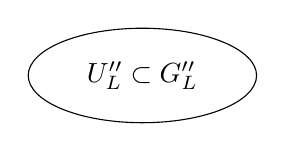
\begin{tikzpicture}
\node at (1.4,0) {$U''_L\subset G''_L$};
\draw (1.4,0) ellipse (1.45 and 0.6);
\end{tikzpicture}}
\uline{défini} par $j_L$. On a un torseur
\inserted{à droite} can (\unsure{uni|mais} trivial)
$\boxed{R_L\text{ sous }U''_L}$, d'où foncteur fibré filtré
\[
\operatorname{DR}_L(M)=\deleted{T_p(M)_L}
(R_L\wedge_{U''_L}Q_L)\wedge_{G_L}T_p(M)_L
\]

\deleted{\unsure{5)}} Le foncteur fibré $\operatorname{DR}_L(M)$ correspond au $G_L$-tors.
\inserted{à dr.}
\figure{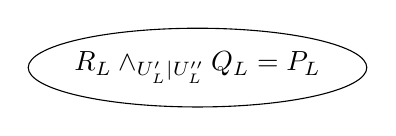
\begin{tikzpicture}
\node at (2,0) {$R_L\wedge_{\unsure{U'_L|U''_L}}Q_L=P_L$};
\draw (2,0) ellipse (2.15 and 0.5);
\end{tikzpicture}}
Soit $\unsure{G''_L|G'_L}=\uline{\operatorname{Aut}}(P_L)$
\[
(G''_L\simeq G'_L\text{ non canonique})
\]

\figure{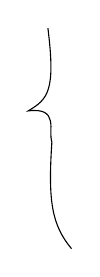
\begin{tikzpicture}[x=1cm,y=1cm]
\draw (0.25,2.8) .. controls (0.35,2) and (0.25,1.9) .. (0,1.75)
 .. controls (0.4,1.8) and (0.25,1.5) .. (0.3,1.35)
 .. controls (0.25,0.6) and (0.3,0.3) .. (0.55,0);
\end{tikzpicture}}
5) \uline{Structure de descente} de $L$ à $K$ \uline{sur le}
\uline{torseur} $P_L$, d'où
\[
\unsure{G''|G'}\quad P_K\quad G_K
\]
6) $G_K$-Isom donné
\[
P_K\simeq P_{\unsure{k|L}}^{(\unsure{f|\phi})}
\]

On peut formuler ensemble 5) et 6) en regardant
\[
P_\Omega=\unsure{R_L^{\leftarrow}|R_L}\wedge_{U''_\Omega}\deleted{\unsure{P}}Q''_\Omega
=R_L\wedge_{U''_\Omega}
\]
et en déclarant que l'ext. $\Gamma$ de $\mathbf Z$ par
$\widetilde\pi=\operatorname{Gal}(\unsure{\bar k/k|\bar K/K})$
(qui contient $\pi\subset\Gamma$) \uline{opère} sur $P_\Omega$ en \unsure{prolongeant}
l'op. \unsure{qu'on a} déjà sur $\pi$.
\margin{26}
